% Options for packages loaded elsewhere
\PassOptionsToPackage{unicode}{hyperref}
\PassOptionsToPackage{hyphens}{url}
\documentclass[
]{article}
\usepackage{xcolor}
\usepackage[margin=1in]{geometry}
\usepackage{amsmath,amssymb}
\setcounter{secnumdepth}{-\maxdimen} % remove section numbering
\usepackage{iftex}
\ifPDFTeX
  \usepackage[T1]{fontenc}
  \usepackage[utf8]{inputenc}
  \usepackage{textcomp} % provide euro and other symbols
\else % if luatex or xetex
  \usepackage{unicode-math} % this also loads fontspec
  \defaultfontfeatures{Scale=MatchLowercase}
  \defaultfontfeatures[\rmfamily]{Ligatures=TeX,Scale=1}
\fi
\usepackage{lmodern}
\ifPDFTeX\else
  % xetex/luatex font selection
\fi
% Use upquote if available, for straight quotes in verbatim environments
\IfFileExists{upquote.sty}{\usepackage{upquote}}{}
\IfFileExists{microtype.sty}{% use microtype if available
  \usepackage[]{microtype}
  \UseMicrotypeSet[protrusion]{basicmath} % disable protrusion for tt fonts
}{}
\makeatletter
\@ifundefined{KOMAClassName}{% if non-KOMA class
  \IfFileExists{parskip.sty}{%
    \usepackage{parskip}
  }{% else
    \setlength{\parindent}{0pt}
    \setlength{\parskip}{6pt plus 2pt minus 1pt}}
}{% if KOMA class
  \KOMAoptions{parskip=half}}
\makeatother
\usepackage{color}
\usepackage{fancyvrb}
\newcommand{\VerbBar}{|}
\newcommand{\VERB}{\Verb[commandchars=\\\{\}]}
\DefineVerbatimEnvironment{Highlighting}{Verbatim}{commandchars=\\\{\}}
% Add ',fontsize=\small' for more characters per line
\usepackage{framed}
\definecolor{shadecolor}{RGB}{248,248,248}
\newenvironment{Shaded}{\begin{snugshade}}{\end{snugshade}}
\newcommand{\AlertTok}[1]{\textcolor[rgb]{0.94,0.16,0.16}{#1}}
\newcommand{\AnnotationTok}[1]{\textcolor[rgb]{0.56,0.35,0.01}{\textbf{\textit{#1}}}}
\newcommand{\AttributeTok}[1]{\textcolor[rgb]{0.13,0.29,0.53}{#1}}
\newcommand{\BaseNTok}[1]{\textcolor[rgb]{0.00,0.00,0.81}{#1}}
\newcommand{\BuiltInTok}[1]{#1}
\newcommand{\CharTok}[1]{\textcolor[rgb]{0.31,0.60,0.02}{#1}}
\newcommand{\CommentTok}[1]{\textcolor[rgb]{0.56,0.35,0.01}{\textit{#1}}}
\newcommand{\CommentVarTok}[1]{\textcolor[rgb]{0.56,0.35,0.01}{\textbf{\textit{#1}}}}
\newcommand{\ConstantTok}[1]{\textcolor[rgb]{0.56,0.35,0.01}{#1}}
\newcommand{\ControlFlowTok}[1]{\textcolor[rgb]{0.13,0.29,0.53}{\textbf{#1}}}
\newcommand{\DataTypeTok}[1]{\textcolor[rgb]{0.13,0.29,0.53}{#1}}
\newcommand{\DecValTok}[1]{\textcolor[rgb]{0.00,0.00,0.81}{#1}}
\newcommand{\DocumentationTok}[1]{\textcolor[rgb]{0.56,0.35,0.01}{\textbf{\textit{#1}}}}
\newcommand{\ErrorTok}[1]{\textcolor[rgb]{0.64,0.00,0.00}{\textbf{#1}}}
\newcommand{\ExtensionTok}[1]{#1}
\newcommand{\FloatTok}[1]{\textcolor[rgb]{0.00,0.00,0.81}{#1}}
\newcommand{\FunctionTok}[1]{\textcolor[rgb]{0.13,0.29,0.53}{\textbf{#1}}}
\newcommand{\ImportTok}[1]{#1}
\newcommand{\InformationTok}[1]{\textcolor[rgb]{0.56,0.35,0.01}{\textbf{\textit{#1}}}}
\newcommand{\KeywordTok}[1]{\textcolor[rgb]{0.13,0.29,0.53}{\textbf{#1}}}
\newcommand{\NormalTok}[1]{#1}
\newcommand{\OperatorTok}[1]{\textcolor[rgb]{0.81,0.36,0.00}{\textbf{#1}}}
\newcommand{\OtherTok}[1]{\textcolor[rgb]{0.56,0.35,0.01}{#1}}
\newcommand{\PreprocessorTok}[1]{\textcolor[rgb]{0.56,0.35,0.01}{\textit{#1}}}
\newcommand{\RegionMarkerTok}[1]{#1}
\newcommand{\SpecialCharTok}[1]{\textcolor[rgb]{0.81,0.36,0.00}{\textbf{#1}}}
\newcommand{\SpecialStringTok}[1]{\textcolor[rgb]{0.31,0.60,0.02}{#1}}
\newcommand{\StringTok}[1]{\textcolor[rgb]{0.31,0.60,0.02}{#1}}
\newcommand{\VariableTok}[1]{\textcolor[rgb]{0.00,0.00,0.00}{#1}}
\newcommand{\VerbatimStringTok}[1]{\textcolor[rgb]{0.31,0.60,0.02}{#1}}
\newcommand{\WarningTok}[1]{\textcolor[rgb]{0.56,0.35,0.01}{\textbf{\textit{#1}}}}
\usepackage{graphicx}
\makeatletter
\newsavebox\pandoc@box
\newcommand*\pandocbounded[1]{% scales image to fit in text height/width
  \sbox\pandoc@box{#1}%
  \Gscale@div\@tempa{\textheight}{\dimexpr\ht\pandoc@box+\dp\pandoc@box\relax}%
  \Gscale@div\@tempb{\linewidth}{\wd\pandoc@box}%
  \ifdim\@tempb\p@<\@tempa\p@\let\@tempa\@tempb\fi% select the smaller of both
  \ifdim\@tempa\p@<\p@\scalebox{\@tempa}{\usebox\pandoc@box}%
  \else\usebox{\pandoc@box}%
  \fi%
}
% Set default figure placement to htbp
\def\fps@figure{htbp}
\makeatother
\setlength{\emergencystretch}{3em} % prevent overfull lines
\providecommand{\tightlist}{%
  \setlength{\itemsep}{0pt}\setlength{\parskip}{0pt}}
\usepackage{bookmark}
\IfFileExists{xurl.sty}{\usepackage{xurl}}{} % add URL line breaks if available
\urlstyle{same}
\hypersetup{
  pdftitle={EDA MyAnimeList},
  pdfauthor={Kacper Janusz},
  hidelinks,
  pdfcreator={LaTeX via pandoc}}

\title{EDA MyAnimeList}
\author{Kacper Janusz}
\date{2026-01-11}

\begin{document}
\maketitle

\subsection{Słowem wstępu}\label{sux142owem-wstux119pu}

Wśród dostępnych treści rozrywkowych w Polsce, coraz większą popularność
zdobywa gatunek ``Anime''.\\
Jest to japoński nurt, w którym tworzone są seriale oraz filmy, których
główną charakterystyczną cechą jest kreowanie opowieści w kreskówkowym
świecie, z bardzo specyficznej stylistyce - nieproporcjonalne wymiary
twarzy, wielkie oczy, kolorowe włosy. W Polsce coraz częściej można się
zetknąć z napływem tytułów filmowych w kinach, wobec czego uznałem, że
jest to doskonała okazja do przebadania społeczności widzów ``anime'',
oraz poszukanie pewnych wzorców i ciekawych insightów na temat
preferencji tej części społeczeństwa.

\subsection{Pochodzenie datasetu}\label{pochodzenie-datasetu}

Wszystkie dane przedstawiane w poniższym arkuszu pochodzą z portalu
MyAnimeList.net.\\
Jest to jeden z największych portali internetowych, który posiada
informacje na temat wszystkich tytułów japońskich seriali rysunkowych,
które były, są i będą wydawane. Na portalu kaggle pojawia się co roku
zestawienie wszystkich tytułów, od najstarszych istniejących rekordów,
aż po te, zgromadzone w roku których dotyczy dataset. Pochodzi ono
dokładnie z danych wyżej wspomnianego serwisu. (Na potrzeby bardziej
wnikliwych analiz, deweloperzy udostępnili również API). Ja w analizie
posłużę się danymi w 2023 roku, z prostego powodu - jest to najlepiej
przygotowany dataset wśród tych z pozostałych lat. Wybrałem ten, który
został przez autora wstępnie przefiltrowany, wobec czego proces
schematyzowania zestawu danych powinien przebiec sprawniej.

\subsection{Wstępna analiza}\label{wstux119pna-analiza}

\begin{Shaded}
\begin{Highlighting}[]
\NormalTok{dataset }\OtherTok{\textless{}{-}} \FunctionTok{read.csv}\NormalTok{(}\StringTok{"anime{-}filtered.csv"}\NormalTok{)}
\FunctionTok{str}\NormalTok{(dataset)}
\end{Highlighting}
\end{Shaded}

\begin{verbatim}
## 'data.frame':    14952 obs. of  25 variables:
##  $ anime_id     : int  1 5 6 7 8 15 16 17 18 19 ...
##  $ Name         : chr  "Cowboy Bebop" "Cowboy Bebop: Tengoku no Tobira" "Trigun" "Witch Hunter Robin" ...
##  $ Score        : num  8.78 8.39 8.24 7.27 6.98 7.95 8.06 7.59 8.15 8.76 ...
##  $ Genres       : chr  "Action, Adventure, Comedy, Drama, Sci-Fi, Space" "Action, Drama, Mystery, Sci-Fi, Space" "Action, Sci-Fi, Adventure, Comedy, Drama, Shounen" "Action, Mystery, Police, Supernatural, Drama, Magic" ...
##  $ English.name : chr  "Cowboy Bebop" "Cowboy Bebop:The Movie" "Trigun" "Witch Hunter Robin" ...
##  $ Japanese.name: chr  "カウボーイビバップ" "カウボーイビバップ 天国の扉" "トライガン" "Witch Hunter ROBIN (ウイッチハンターロビン)" ...
##  $ sypnopsis    : chr  "In the year 2071, humanity has colonized several of the planets and moons of the solar system leaving the now u"| __truncated__ "other day, another bounty—such is the life of the often unlucky crew of the Bebop. However, this routine is int"| __truncated__ "Vash the Stampede is the man with a $$60,000,000,000 bounty on his head. The reason: he's a merciless villain w"| __truncated__ "ches are individuals with special powers like ESP, telekinesis, mind control, etc. Robin, a 15-year-old craft u"| __truncated__ ...
##  $ Type         : chr  "TV" "Movie" "TV" "TV" ...
##  $ Episodes     : chr  "26" "1" "26" "26" ...
##  $ Aired        : chr  "Apr 3, 1998 to Apr 24, 1999" "Sep 1, 2001" "Apr 1, 1998 to Sep 30, 1998" "Jul 2, 2002 to Dec 24, 2002" ...
##  $ Premiered    : chr  "Spring 1998" "Unknown" "Spring 1998" "Summer 2002" ...
##  $ Producers    : chr  "Bandai Visual" "Sunrise, Bandai Visual" "Victor Entertainment" "TV Tokyo, Bandai Visual, Dentsu, Victor Entertainment" ...
##  $ Licensors    : chr  "Funimation, Bandai Entertainment" "Sony Pictures Entertainment" "Funimation, Geneon Entertainment USA" "Funimation, Bandai Entertainment" ...
##  $ Studios      : chr  "Sunrise" "Bones" "Madhouse" "Sunrise" ...
##  $ Source       : chr  "Original" "Original" "Manga" "Original" ...
##  $ Duration     : chr  "24 min. per ep." "1 hr. 55 min." "24 min. per ep." "25 min. per ep." ...
##  $ Rating       : chr  "R - 17+ (violence & profanity)" "R - 17+ (violence & profanity)" "PG-13 - Teens 13 or older" "PG-13 - Teens 13 or older" ...
##  $ Ranked       : num  28 159 266 2481 3710 ...
##  $ Popularity   : int  39 518 201 1467 4369 1003 687 3612 1233 169 ...
##  $ Members      : int  1251960 273145 558913 94683 13224 148259 214499 20470 117929 614100 ...
##  $ Favorites    : int  61971 1174 12944 587 18 2066 4101 231 979 29436 ...
##  $ Watching     : int  105808 4143 29113 4300 642 13907 11909 817 6082 64648 ...
##  $ Completed    : int  718161 208333 343492 46165 7314 78349 81145 13778 90967 214491 ...
##  $ On.Hold      : int  71513 1935 25465 5121 766 14228 11901 828 3053 47488 ...
##  $ Dropped      : int  26678 770 13925 5378 1108 11573 11026 1168 1356 23008 ...
\end{verbatim}

Nasz dataset składa się w sumie z 25 kolumn i 14952 rekordów. Może się
to wydawać kolosalna liczba w konteście skali tej analizy, jednak sądzę,
że w tym przypadku dobrze jest mieć jak najwięcej datapointów -
potencjalne korelacje będą na większej próbie.

\begin{Shaded}
\begin{Highlighting}[]
\FunctionTok{summary}\NormalTok{(dataset)}
\end{Highlighting}
\end{Shaded}

\begin{verbatim}
##     anime_id         Name               Score          Genres         
##  Min.   :    1   Length:14952       Min.   :1.850   Length:14952      
##  1st Qu.: 4602   Class :character   1st Qu.:6.080   Class :character  
##  Median :16729   Mode  :character   Median :6.510   Mode  :character  
##  Mean   :19017                      Mean   :6.512                     
##  3rd Qu.:33513                      3rd Qu.:7.010                     
##  Max.   :48492                      Max.   :9.190                     
##                                                                       
##  English.name       Japanese.name       sypnopsis             Type          
##  Length:14952       Length:14952       Length:14952       Length:14952      
##  Class :character   Class :character   Class :character   Class :character  
##  Mode  :character   Mode  :character   Mode  :character   Mode  :character  
##                                                                             
##                                                                             
##                                                                             
##                                                                             
##    Episodes            Aired            Premiered          Producers        
##  Length:14952       Length:14952       Length:14952       Length:14952      
##  Class :character   Class :character   Class :character   Class :character  
##  Mode  :character   Mode  :character   Mode  :character   Mode  :character  
##                                                                             
##                                                                             
##                                                                             
##                                                                             
##   Licensors           Studios             Source            Duration        
##  Length:14952       Length:14952       Length:14952       Length:14952      
##  Class :character   Class :character   Class :character   Class :character  
##  Mode  :character   Mode  :character   Mode  :character   Mode  :character  
##                                                                             
##                                                                             
##                                                                             
##                                                                             
##     Rating              Ranked        Popularity       Members       
##  Length:14952       Min.   :    1   Min.   :    1   Min.   :    200  
##  Class :character   1st Qu.: 3310   1st Qu.: 3732   1st Qu.:    736  
##  Mode  :character   Median : 6618   Median : 7466   Median :   3494  
##                     Mean   : 6830   Mean   : 7466   Mean   :  40686  
##                     3rd Qu.: 9942   3rd Qu.:11194   3rd Qu.:  19193  
##                     Max.   :15780   Max.   :17565   Max.   :2589552  
##                     NA's   :1721                                     
##    Favorites           Watching        Completed          On.Hold        
##  Min.   :     0.0   Min.   :     0   Min.   :      0   Min.   :     0.0  
##  1st Qu.:     1.0   1st Qu.:    27   1st Qu.:    246   1st Qu.:    14.0  
##  Median :     6.0   Median :   127   Median :   1516   Median :    78.0  
##  Mean   :   537.6   Mean   :  2620   Mean   :  25943   Mean   :  1121.3  
##  3rd Qu.:    47.0   3rd Qu.:   723   3rd Qu.:   9797   3rd Qu.:   388.2  
##  Max.   :183914.0   Max.   :887333   Max.   :2182587   Max.   :187919.0  
##                                                                          
##     Dropped      
##  Min.   :     0  
##  1st Qu.:    48  
##  Median :   102  
##  Mean   :  1378  
##  3rd Qu.:   377  
##  Max.   :174710  
## 
\end{verbatim}

\subsubsection{Opis kolumn}\label{opis-kolumn}

Mamy 25 kolumn, w których mamy dane ilościowe, jakościowe, oraz widać od
razu, że pewne z nich doskonale byłoby przekonwertować na factory.\\
Kolumny ``anime\_id'', ``Name'', ``English.name'', ``Japanese.name'' to
kolumny, które pomagają rozpoznać, o który tytuł dokładnie chodzi. Nie
potrzebujemy ich wszystkich na potrzeby naszej analizy, postanowiłem
zostawić wyłącznie ``English.name'' które pozostanie pod nazwą ``Name''

\begin{Shaded}
\begin{Highlighting}[]
\NormalTok{dataset}\SpecialCharTok{$}\NormalTok{Japanese.name }\OtherTok{\textless{}{-}} \ConstantTok{NULL}
\NormalTok{dataset}\SpecialCharTok{$}\NormalTok{anime\_id }\OtherTok{\textless{}{-}} \ConstantTok{NULL}
\NormalTok{dataset}\SpecialCharTok{$}\NormalTok{Name }\OtherTok{\textless{}{-}}\NormalTok{ dataset}\SpecialCharTok{$}\NormalTok{English.name}
\NormalTok{dataset}\SpecialCharTok{$}\NormalTok{English.name }\OtherTok{\textless{}{-}} \ConstantTok{NULL}
\end{Highlighting}
\end{Shaded}

Kolumna ``Synopsis'' to streszczenie konkretnego tytułu, na ten moment
nie znajduję przyczyny, aby ją pozostawić. Potencjalnie możnaby dokonać
analizy, jak bardzo emocjonalne są powyższe opisy i jak bardzo mogą
wpływać na opinię oglądających, jednak pozostawiam ten temat jako
opcjonalny na później.

\begin{Shaded}
\begin{Highlighting}[]
\NormalTok{dataset}\SpecialCharTok{$}\NormalTok{sypnopsis }\OtherTok{\textless{}{-}} \ConstantTok{NULL}
\end{Highlighting}
\end{Shaded}

Kolumny ``Type'', ``Episodes'', ``Aired'', ``Premiered'', ``Duration'',
``Rating'' odnoszą się typowo do okresu release'u produkcji, czyli mówią
nam w skrócie: Gdzie, kiedy, i w ilu odcinkach był emitowany
serial/film, ile trwał każdy z odcinków, jakie miał ograniczenia wiekowe
oraz kiedy pojawiła się w ogóle pierwsza oficjalna wzmianka o nim.

``Source'' oznacza, czy produkcja jest bazowana na opowieści z książki,
czy też jest to oryginalna fabuła.

Mamy również dosępne kilka kolumn, dzięki którym będzie można stworzyć
charakterystykę wypuszczanych anime przez konkretne studia ``Studios'',
wydawców ``Licensors'' oraz producentów ``Producers.

Następna grupa wartości związana jest już stricte ze społecznością fanów
anime, ponieważ kolumny ``Ranked'', ``Score'' oraz ``Popularity''
odpowiadają kolejno za miejsce w tabeli najlepszych tytułów, średni
wynik punktowy oraz miejsce w tabeli tytułów, które najczęściej były
oglądane i oceniane.

Ostatnia grupa kolumn, to te mówiące o zachowaniu widzów: ``Members''
mówi dokładnie ile osób oceniło/obejrzało/jakkolwiek ``ruszyło'' daną
produkcję, ``Favorites'' to dla ilu produkcja znajduje się w kategorii
``ulubione'', ``Watching'' to ile osób obecnie ogląda dany tytuł (na co
trzeba brać poprawkę ponieważ w wielu przypadkach użytkownicy nie
odznaczają obejrzanych już tytułów), ``Completed'' jako ukończony tytuł,
``On.Hold'' oznacza, że osoba wstrzymała oglądanie, a ``Dropped'' to
metryka mówiąca ile osób nie skończyło sezonu/filmu, porzucając
zakończenie wraz z puentą całego tytułu.

Najważniejszą z nich jednak zostawiłem na koniec - ``Genre'', czyli
gatunek. Moim zdaniem będzie to bardzo przydatna informacja podczas
analizy preferencji użytkowników. Wierzę, że uda się z niej wyciągnąć
najwięcej spostrzeżeń.

\begin{Shaded}
\begin{Highlighting}[]
\FunctionTok{library}\NormalTok{(mice)}
\FunctionTok{md.pattern}\NormalTok{(dataset)}
\end{Highlighting}
\end{Shaded}

\pandocbounded{\includegraphics[keepaspectratio]{EDA_files/figure-latex/unnamed-chunk-4-1.pdf}}

\begin{verbatim}
##       Name Score Genres Type Episodes Aired Premiered Producers Licensors
## 13231    1     1      1    1        1     1         1         1         1
## 1721     1     1      1    1        1     1         1         1         1
##          0     0      0    0        0     0         0         0         0
##       Studios Source Duration Rating Popularity Members Favorites Watching
## 13231       1      1        1      1          1       1         1        1
## 1721        1      1        1      1          1       1         1        1
##             0      0        0      0          0       0         0        0
##       Completed On.Hold Dropped Ranked     
## 13231         1       1       1      1    0
## 1721          1       1       1      0    1
##               0       0       0   1721 1721
\end{verbatim}

\subsection{Braki danych}\label{braki-danych}

Przefiltrowany dataset posiada przeszło 14 tysięcy rekordów, a mimo to
zdarzyły się takie, które nie posiadają pewnych informacji. ``Rating''
to jednak kategoria wiekowa, więc można przypuszczać, że są seriale,
które nie miały przyznanej żadnej kategorii, być może przez to, że
jeszcze nie wyszły, a może właśnie dlatego, że są tak stare.
Postanowiłem zostawić te tytuły i zachować ostrożność podczas filtracji.

\subsection{Porządkowanie struktury
datasetu}\label{porzux105dkowanie-struktury-datasetu}

Przechodzę do konwersji arkusza do postaci, w której będę mógł nim
swobodnie manipulować Mam kolumny, które wprost proszą się o konwersję
na factor.

\begin{Shaded}
\begin{Highlighting}[]
\FunctionTok{table}\NormalTok{(dataset}\SpecialCharTok{$}\NormalTok{Type)}
\end{Highlighting}
\end{Shaded}

\begin{verbatim}
## 
##   Movie   Music     ONA     OVA Special      TV Unknown 
##    2636     744    1531    3364    1991    4650      36
\end{verbatim}

\begin{Shaded}
\begin{Highlighting}[]
\NormalTok{dataset}\SpecialCharTok{$}\NormalTok{Type }\OtherTok{\textless{}{-}} \FunctionTok{as.factor}\NormalTok{(dataset}\SpecialCharTok{$}\NormalTok{Type)}
\FunctionTok{table}\NormalTok{(dataset}\SpecialCharTok{$}\NormalTok{Source)}
\end{Highlighting}
\end{Shaded}

\begin{verbatim}
## 
##  4-koma manga          Book     Card game Digital manga          Game 
##           277            87            64            15           829 
##   Light novel         Manga         Music         Novel      Original 
##           768          3764           215           485          3720 
##         Other  Picture book         Radio       Unknown  Visual novel 
##           444            76             9          2974           988 
##     Web manga 
##           237
\end{verbatim}

\begin{Shaded}
\begin{Highlighting}[]
\NormalTok{dataset}\SpecialCharTok{$}\NormalTok{Source }\OtherTok{\textless{}{-}} \FunctionTok{as.factor}\NormalTok{(dataset}\SpecialCharTok{$}\NormalTok{Source)}
\end{Highlighting}
\end{Shaded}

Ale mam też takie, które choć bym chciał, nie jestem w stanie
przekształcić w nieinwazyjny sposób. Kolumny takie jak:

\begin{Shaded}
\begin{Highlighting}[]
\FunctionTok{length}\NormalTok{(}\FunctionTok{unique}\NormalTok{(dataset}\SpecialCharTok{$}\NormalTok{Studios))}
\end{Highlighting}
\end{Shaded}

\begin{verbatim}
## [1] 1048
\end{verbatim}

\begin{Shaded}
\begin{Highlighting}[]
\FunctionTok{length}\NormalTok{(dataset}\SpecialCharTok{$}\NormalTok{Studios)}
\end{Highlighting}
\end{Shaded}

\begin{verbatim}
## [1] 14952
\end{verbatim}

\begin{Shaded}
\begin{Highlighting}[]
\FunctionTok{length}\NormalTok{(}\FunctionTok{unique}\NormalTok{(dataset}\SpecialCharTok{$}\NormalTok{Producers))}
\end{Highlighting}
\end{Shaded}

\begin{verbatim}
## [1] 3714
\end{verbatim}

\begin{Shaded}
\begin{Highlighting}[]
\FunctionTok{length}\NormalTok{(dataset}\SpecialCharTok{$}\NormalTok{Producers)}
\end{Highlighting}
\end{Shaded}

\begin{verbatim}
## [1] 14952
\end{verbatim}

\begin{Shaded}
\begin{Highlighting}[]
\FunctionTok{length}\NormalTok{(}\FunctionTok{unique}\NormalTok{(dataset}\SpecialCharTok{$}\NormalTok{Licensors))}
\end{Highlighting}
\end{Shaded}

\begin{verbatim}
## [1] 231
\end{verbatim}

\begin{Shaded}
\begin{Highlighting}[]
\FunctionTok{length}\NormalTok{(dataset}\SpecialCharTok{$}\NormalTok{Licensors)}
\end{Highlighting}
\end{Shaded}

\begin{verbatim}
## [1] 14952
\end{verbatim}

Pasowałyby jako factor, ale tych wartości jest zbyt wiele, blisko 9-15\%
całego datasetu, więc pozostawiam je jako napis.

I szczególnie ta, w której pokładam najwięcej nadziei:

\begin{Shaded}
\begin{Highlighting}[]
\FunctionTok{head}\NormalTok{(dataset}\SpecialCharTok{$}\NormalTok{Genres)}
\end{Highlighting}
\end{Shaded}

\begin{verbatim}
## [1] "Action, Adventure, Comedy, Drama, Sci-Fi, Space"    
## [2] "Action, Drama, Mystery, Sci-Fi, Space"              
## [3] "Action, Sci-Fi, Adventure, Comedy, Drama, Shounen"  
## [4] "Action, Mystery, Police, Supernatural, Drama, Magic"
## [5] "Adventure, Fantasy, Shounen, Supernatural"          
## [6] "Action, Sports, Comedy, Shounen"
\end{verbatim}

\begin{Shaded}
\begin{Highlighting}[]
\FunctionTok{length}\NormalTok{(}\FunctionTok{unique}\NormalTok{(dataset}\SpecialCharTok{$}\NormalTok{Genres))}
\end{Highlighting}
\end{Shaded}

\begin{verbatim}
## [1] 4839
\end{verbatim}

Posiada one wiele rekordów rodzielonych przecinkami, więc zdecydowałem
się na potrzeby badań, zbudować funkcję, która zadziała na zasadzie
``LIKE \% \%'' w SQL. To pozwoli mi bez większych problemów mimo
wszystko odszukać rekordy, które zawierają nie tylko tą kategorię, po
której filtruję (oraz posłużą również do Procudentów, Wydawców i
Studiów)

\begin{Shaded}
\begin{Highlighting}[]
\NormalTok{like }\OtherTok{\textless{}{-}} \ControlFlowTok{function}\NormalTok{(text, searched\_string)\{}
\NormalTok{  words }\OtherTok{\textless{}{-}} \FunctionTok{strsplit}\NormalTok{(text, }\StringTok{","}\NormalTok{)[[}\DecValTok{1}\NormalTok{]]}
\NormalTok{  words }\OtherTok{\textless{}{-}} \FunctionTok{trimws}\NormalTok{(words)}
  \FunctionTok{return}\NormalTok{(searched\_string }\SpecialCharTok{\%in\%}\NormalTok{ words)}
\NormalTok{\}}
\end{Highlighting}
\end{Shaded}

Funkcja zakłada, że po przecinkach będzie znajdować się dokładnie takie
słowo, jakiego szukamy, nie przyjmuje niestety wycinków nazw podobnie
jak LIKE w SQL, jednak dobrze, że w ogóle mogę się z tym w ten sposób
uporać.

Finalny kształt datasetu:

\begin{Shaded}
\begin{Highlighting}[]
\FunctionTok{str}\NormalTok{(dataset)}
\end{Highlighting}
\end{Shaded}

\begin{verbatim}
## 'data.frame':    14952 obs. of  21 variables:
##  $ Name      : chr  "Cowboy Bebop" "Cowboy Bebop:The Movie" "Trigun" "Witch Hunter Robin" ...
##  $ Score     : num  8.78 8.39 8.24 7.27 6.98 7.95 8.06 7.59 8.15 8.76 ...
##  $ Genres    : chr  "Action, Adventure, Comedy, Drama, Sci-Fi, Space" "Action, Drama, Mystery, Sci-Fi, Space" "Action, Sci-Fi, Adventure, Comedy, Drama, Shounen" "Action, Mystery, Police, Supernatural, Drama, Magic" ...
##  $ Type      : Factor w/ 7 levels "Movie","Music",..: 6 1 6 6 6 6 6 6 6 6 ...
##  $ Episodes  : chr  "26" "1" "26" "26" ...
##  $ Aired     : chr  "Apr 3, 1998 to Apr 24, 1999" "Sep 1, 2001" "Apr 1, 1998 to Sep 30, 1998" "Jul 2, 2002 to Dec 24, 2002" ...
##  $ Premiered : chr  "Spring 1998" "Unknown" "Spring 1998" "Summer 2002" ...
##  $ Producers : chr  "Bandai Visual" "Sunrise, Bandai Visual" "Victor Entertainment" "TV Tokyo, Bandai Visual, Dentsu, Victor Entertainment" ...
##  $ Licensors : chr  "Funimation, Bandai Entertainment" "Sony Pictures Entertainment" "Funimation, Geneon Entertainment USA" "Funimation, Bandai Entertainment" ...
##  $ Studios   : chr  "Sunrise" "Bones" "Madhouse" "Sunrise" ...
##  $ Source    : Factor w/ 16 levels "4-koma manga",..: 10 10 7 10 7 7 7 7 7 7 ...
##  $ Duration  : chr  "24 min. per ep." "1 hr. 55 min." "24 min. per ep." "25 min. per ep." ...
##  $ Rating    : chr  "R - 17+ (violence & profanity)" "R - 17+ (violence & profanity)" "PG-13 - Teens 13 or older" "PG-13 - Teens 13 or older" ...
##  $ Ranked    : num  28 159 266 2481 3710 ...
##  $ Popularity: int  39 518 201 1467 4369 1003 687 3612 1233 169 ...
##  $ Members   : int  1251960 273145 558913 94683 13224 148259 214499 20470 117929 614100 ...
##  $ Favorites : int  61971 1174 12944 587 18 2066 4101 231 979 29436 ...
##  $ Watching  : int  105808 4143 29113 4300 642 13907 11909 817 6082 64648 ...
##  $ Completed : int  718161 208333 343492 46165 7314 78349 81145 13778 90967 214491 ...
##  $ On.Hold   : int  71513 1935 25465 5121 766 14228 11901 828 3053 47488 ...
##  $ Dropped   : int  26678 770 13925 5378 1108 11573 11026 1168 1356 23008 ...
\end{verbatim}

\subsection{Wstępna analiza}\label{wstux119pna-analiza-1}

\subsubsection{Score}\label{score}

Przechodzę do wstępnej analizy liczb, dostępnych w naszym datasecie.\\
Na pierwszy ogień przeanalizuję końcową ocenę użytkowników, dzięki czemu
dowiemy się, w jakim zakresie (0-10) wystawiane są najchętniej oceny

\begin{Shaded}
\begin{Highlighting}[]
\FunctionTok{library}\NormalTok{(ggplot2)}

\FunctionTok{min}\NormalTok{(dataset}\SpecialCharTok{$}\NormalTok{Score)}
\end{Highlighting}
\end{Shaded}

\begin{verbatim}
## [1] 1.85
\end{verbatim}

\begin{Shaded}
\begin{Highlighting}[]
\FunctionTok{max}\NormalTok{(dataset}\SpecialCharTok{$}\NormalTok{Score)}
\end{Highlighting}
\end{Shaded}

\begin{verbatim}
## [1] 9.19
\end{verbatim}

Dane wahają nam się od 1.85 do 9.19, więc biorąc pod uwagę skalę 10-cio
stopniową, nie mamy pełnej rozpiętości danych. To wskazuje, że nie ma
tytułów, które byłyby jednogłośnie okrzyknięte arcydziełem, ani też
tragicznych produkcji. Mimo to, są ekstrema i na pewno coś kierowało
odbiorcami, żeby tak ocenić dane anime.

\begin{Shaded}
\begin{Highlighting}[]
\FunctionTok{mean}\NormalTok{(dataset}\SpecialCharTok{$}\NormalTok{Score)}
\end{Highlighting}
\end{Shaded}

\begin{verbatim}
## [1] 6.511526
\end{verbatim}

\begin{Shaded}
\begin{Highlighting}[]
\FunctionTok{median}\NormalTok{(dataset}\SpecialCharTok{$}\NormalTok{Score)}
\end{Highlighting}
\end{Shaded}

\begin{verbatim}
## [1] 6.51
\end{verbatim}

Średnia i mediana znajdują się z drobnym błędem dokładnie w tym samym
punkcie. Mamy tutaj idealną symetrię? Ciekawa sprawa, zobaczmy rozkład
tej zmiennej.

\begin{Shaded}
\begin{Highlighting}[]
\FunctionTok{ggplot}\NormalTok{(dataset, }\FunctionTok{aes}\NormalTok{(}\AttributeTok{x=}\NormalTok{dataset}\SpecialCharTok{$}\NormalTok{Score))}\SpecialCharTok{+}
  \FunctionTok{geom\_histogram}\NormalTok{(}\AttributeTok{binwidth=}\NormalTok{.}\DecValTok{1}\NormalTok{)}
\end{Highlighting}
\end{Shaded}

\pandocbounded{\includegraphics[keepaspectratio]{EDA_files/figure-latex/unnamed-chunk-11-1.pdf}}

\begin{Shaded}
\begin{Highlighting}[]
\FunctionTok{ggplot}\NormalTok{(dataset, }\FunctionTok{aes}\NormalTok{(}\AttributeTok{x=}\NormalTok{dataset}\SpecialCharTok{$}\NormalTok{Score))}\SpecialCharTok{+}
  \FunctionTok{geom\_histogram}\NormalTok{(}\AttributeTok{binwidth=}\NormalTok{.}\DecValTok{1}\NormalTok{)}\SpecialCharTok{+}
  \FunctionTok{xlim}\NormalTok{(}\DecValTok{5}\NormalTok{, }\DecValTok{7}\NormalTok{)}
\end{Highlighting}
\end{Shaded}

\pandocbounded{\includegraphics[keepaspectratio]{EDA_files/figure-latex/unnamed-chunk-11-2.pdf}}

I sprawa staje się jasna. Pierwszy rzut oka wskazuje nam dwie rzeczy -
jest widoczny delikatny rozkład z centrum oscylującym wokół 6.7,
natomiast jest też punkt 6.5 który zdaje się być gigantyczną odstającą
daną. To tłumaczy skąd mediana i średnia mają taką wartość. Na tą
potrzebę mogę spróbować ustawić skalę Y jako logarytmiczną

\begin{Shaded}
\begin{Highlighting}[]
\FunctionTok{library}\NormalTok{(ggplot2)}
\FunctionTok{ggplot}\NormalTok{(dataset, }\FunctionTok{aes}\NormalTok{(}\AttributeTok{x=}\NormalTok{dataset}\SpecialCharTok{$}\NormalTok{Score))}\SpecialCharTok{+}
  \FunctionTok{geom\_histogram}\NormalTok{(}\AttributeTok{binwidth=}\NormalTok{.}\DecValTok{1}\NormalTok{)}\SpecialCharTok{+}
  \FunctionTok{scale\_y\_log10}\NormalTok{()}
\end{Highlighting}
\end{Shaded}

\pandocbounded{\includegraphics[keepaspectratio]{EDA_files/figure-latex/unnamed-chunk-12-1.pdf}}

Teraz lepiej widac rozkład danych nieodstających. Warto byłoby
sprawdzić, o co chodzi z tym punktem 6.5. Odfiltruję zakres od 6.4 do
6.6 aby być pewnym, że złapiemy wszystkie, które otaczają 6.5 i wyznaczę
im wskaźniki pozycyjne.

\begin{Shaded}
\begin{Highlighting}[]
\FunctionTok{library}\NormalTok{(dplyr)}
\NormalTok{odstajace }\OtherTok{\textless{}{-}}\NormalTok{ dataset }\SpecialCharTok{\%\textgreater{}\%}
  \FunctionTok{filter}\NormalTok{(dataset}\SpecialCharTok{$}\NormalTok{Score }\SpecialCharTok{\textgreater{}=} \FloatTok{6.4} \SpecialCharTok{\&}\NormalTok{ dataset}\SpecialCharTok{$}\NormalTok{Score }\SpecialCharTok{\textless{}=} \FloatTok{6.6}\NormalTok{)}
\FunctionTok{summary}\NormalTok{(odstajace}\SpecialCharTok{$}\NormalTok{Ranked)}
\end{Highlighting}
\end{Shaded}

\begin{verbatim}
##    Min. 1st Qu.  Median    Mean 3rd Qu.    Max.    NA's 
##    5343    6172   12227   10914   13978   15780     516
\end{verbatim}

Biorąc pod uwagę wartość popularności (im niższa tym wyżej w rankingu =
popularniejszy tytuł), mediana pokazuje, że znaczna część danych jest w
okolicy trzeciego kwartyla, wobec czego można wnioskować, że rozkład ma
skośność lewostronną, ale zweryfikujemy to sobie

\begin{Shaded}
\begin{Highlighting}[]
\FunctionTok{ggplot}\NormalTok{(odstajace, }\FunctionTok{aes}\NormalTok{(}\AttributeTok{y=}\NormalTok{odstajace}\SpecialCharTok{$}\NormalTok{Ranked, }\AttributeTok{x=}\NormalTok{odstajace}\SpecialCharTok{$}\NormalTok{Score))}\SpecialCharTok{+}
  \FunctionTok{geom\_line}\NormalTok{()}
\end{Highlighting}
\end{Shaded}

\pandocbounded{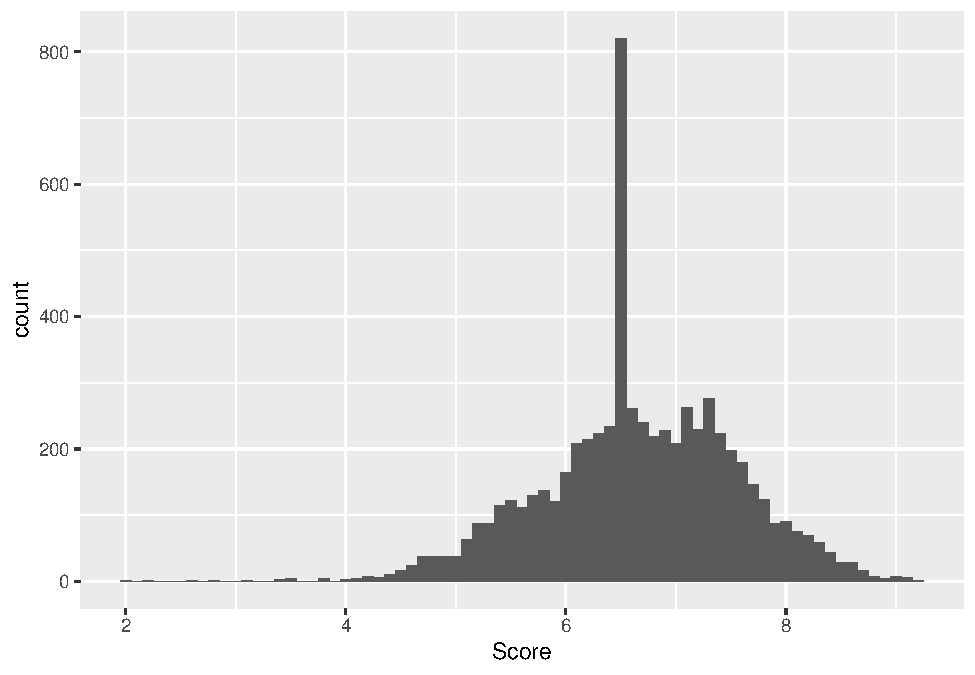
\includegraphics[keepaspectratio]{EDA_files/figure-latex/unnamed-chunk-14-1.pdf}}

Czyli wychodzi na to, że dla wyniku \textasciitilde6,51 jest
nienaturalna liczba rekordów, które co więcej znajdują się w ogonie
całego zbioru w liczbie około 3000. Być może jest to wartość domyślna,
przypisywana automatycznie? Nie wygląda to bynajmniej naturalnie i ja
traktuję to jako daną odstającą. Poniższe badania przeprowadzę na grupie
odfiltrowanej z tego zakresu

\begin{Shaded}
\begin{Highlighting}[]
\NormalTok{filtered }\OtherTok{\textless{}{-}}\NormalTok{ dataset }\SpecialCharTok{\%\textgreater{}\%}
  \FunctionTok{filter}\NormalTok{(dataset}\SpecialCharTok{$}\NormalTok{Score }\SpecialCharTok{\textless{}=} \FloatTok{6.5} \SpecialCharTok{|}\NormalTok{ dataset}\SpecialCharTok{$}\NormalTok{Score }\SpecialCharTok{\textgreater{}=} \FloatTok{6.52}\NormalTok{)}

\FunctionTok{mean}\NormalTok{(filtered}\SpecialCharTok{$}\NormalTok{Score)}
\end{Highlighting}
\end{Shaded}

\begin{verbatim}
## [1] 6.51185
\end{verbatim}

\begin{Shaded}
\begin{Highlighting}[]
\FunctionTok{median}\NormalTok{(filtered}\SpecialCharTok{$}\NormalTok{Score)}
\end{Highlighting}
\end{Shaded}

\begin{verbatim}
## [1] 6.53
\end{verbatim}

\begin{Shaded}
\begin{Highlighting}[]
\FunctionTok{sd}\NormalTok{(filtered}\SpecialCharTok{$}\NormalTok{Score)}
\end{Highlighting}
\end{Shaded}

\begin{verbatim}
## [1] 0.8888103
\end{verbatim}

\begin{Shaded}
\begin{Highlighting}[]
\FunctionTok{var}\NormalTok{(filtered}\SpecialCharTok{$}\NormalTok{Score)}
\end{Highlighting}
\end{Shaded}

\begin{verbatim}
## [1] 0.7899837
\end{verbatim}

\begin{Shaded}
\begin{Highlighting}[]
\FunctionTok{ggplot}\NormalTok{(filtered, }\FunctionTok{aes}\NormalTok{(}\AttributeTok{x=}\NormalTok{filtered}\SpecialCharTok{$}\NormalTok{Score))}\SpecialCharTok{+}
  \FunctionTok{geom\_histogram}\NormalTok{(}\AttributeTok{binwidth=}\NormalTok{.}\DecValTok{1}\NormalTok{)}
\end{Highlighting}
\end{Shaded}

\pandocbounded{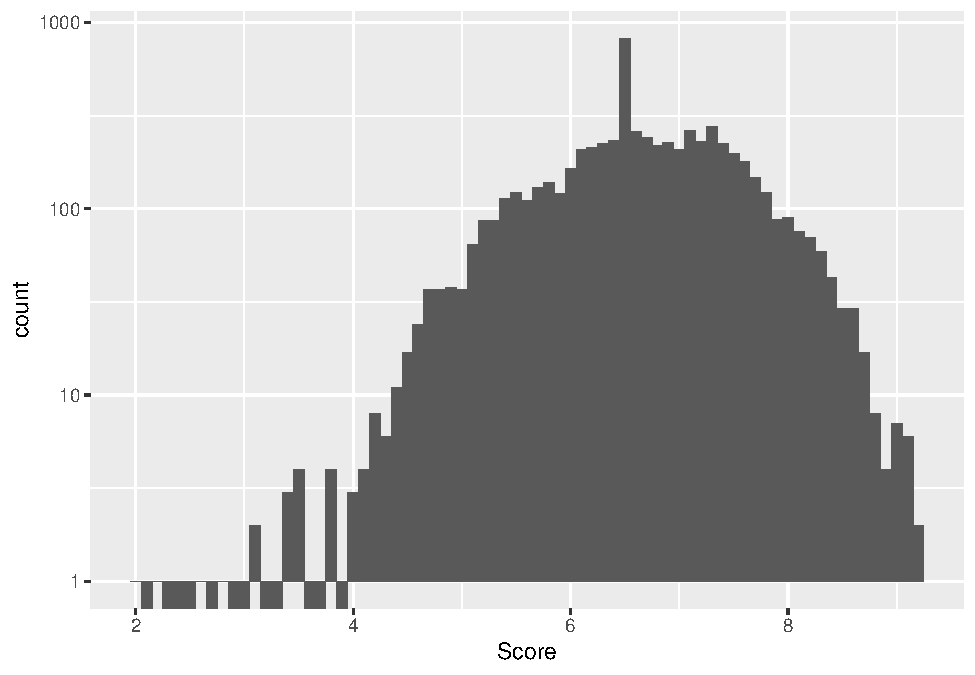
\includegraphics[keepaspectratio]{EDA_files/figure-latex/unnamed-chunk-15-1.pdf}}

Ciekawy wniosek: Mimo usunięcia kompletnie zakresu z odstającymi
wartościami, mediana wyszła bardzo zbliżona. Jest wyższa od średniej co
każde wnioskować, że skośność również jest lewostronna, ale minimalna.
Rozkład ma teraz kształt, który można porównać do rozkładu normalnego.
Jaka obserwacja się nasuwa? Użytkownicy chętnie oceniają produkcje ponad
połowę skali, i są to głównie wartości w przedziale 5-9 punktów. Rozkład
ma wybicie nieco ponad wynikiem 7 gwiazdek (ponieważ to jednostka
stosowana w MAL'u), co może wskazywać, że ludzie mają tendencję do
traktowania siódemki jako taki ``złoty środek'' - nie jest to tytuł
wybitny, nie jest on średni, jest dobry, w sam raz pomiędzy 5 a 9,
ponieważ 10 to już byłoby arcydzieło. Wariancja i odchylenie w granicy
jedynki, mamy tutaj dane skupione wokół centrum o niskiej zmienności.

\subsubsection{Type}\label{type}

Zerknijmy na jedną z naszych zmiennych factorowych

\begin{Shaded}
\begin{Highlighting}[]
\FunctionTok{table}\NormalTok{(dataset}\SpecialCharTok{$}\NormalTok{Type)}
\end{Highlighting}
\end{Shaded}

\begin{verbatim}
## 
##   Movie   Music     ONA     OVA Special      TV Unknown 
##    2636     744    1531    3364    1991    4650      36
\end{verbatim}

\begin{Shaded}
\begin{Highlighting}[]
\NormalTok{filtered }\SpecialCharTok{\%\textgreater{}\%}
  \FunctionTok{filter}\NormalTok{(filtered}\SpecialCharTok{$}\NormalTok{Type }\SpecialCharTok{==} \StringTok{"Movie"}\NormalTok{) }\SpecialCharTok{\%\textgreater{}\%}
  \FunctionTok{summarise}\NormalTok{(}\FunctionTok{median}\NormalTok{(filtered}\SpecialCharTok{$}\NormalTok{Score)) }\SpecialCharTok{\%\textgreater{}\%}
  \FunctionTok{summarise}\NormalTok{(}\FunctionTok{max}\NormalTok{(filtered}\SpecialCharTok{$}\NormalTok{Score))}
\end{Highlighting}
\end{Shaded}

\begin{verbatim}
##   max(filtered$Score)
## 1                9.19
\end{verbatim}

\begin{Shaded}
\begin{Highlighting}[]
\NormalTok{filtered }\SpecialCharTok{\%\textgreater{}\%}
  \FunctionTok{filter}\NormalTok{(filtered}\SpecialCharTok{$}\NormalTok{Type }\SpecialCharTok{==} \StringTok{"TV"}\NormalTok{) }\SpecialCharTok{\%\textgreater{}\%}
  \FunctionTok{summarise}\NormalTok{(}\FunctionTok{median}\NormalTok{(filtered}\SpecialCharTok{$}\NormalTok{Score))}
\end{Highlighting}
\end{Shaded}

\begin{verbatim}
##   median(filtered$Score)
## 1                   6.53
\end{verbatim}

\begin{Shaded}
\begin{Highlighting}[]
\NormalTok{filtered }\SpecialCharTok{\%\textgreater{}\%}
  \FunctionTok{filter}\NormalTok{(filtered}\SpecialCharTok{$}\NormalTok{Type }\SpecialCharTok{==} \StringTok{"OVA"}\NormalTok{) }\SpecialCharTok{\%\textgreater{}\%}
  \FunctionTok{summarise}\NormalTok{(}\FunctionTok{median}\NormalTok{(filtered}\SpecialCharTok{$}\NormalTok{Score))}
\end{Highlighting}
\end{Shaded}

\begin{verbatim}
##   median(filtered$Score)
## 1                   6.53
\end{verbatim}

\begin{Shaded}
\begin{Highlighting}[]
\NormalTok{filtered }\SpecialCharTok{\%\textgreater{}\%}
  \FunctionTok{filter}\NormalTok{(filtered}\SpecialCharTok{$}\NormalTok{Type }\SpecialCharTok{==} \StringTok{"ONA"}\NormalTok{) }\SpecialCharTok{\%\textgreater{}\%}
  \FunctionTok{summarise}\NormalTok{(}\FunctionTok{median}\NormalTok{(filtered}\SpecialCharTok{$}\NormalTok{Score))}
\end{Highlighting}
\end{Shaded}

\begin{verbatim}
##   median(filtered$Score)
## 1                   6.53
\end{verbatim}

\begin{Shaded}
\begin{Highlighting}[]
\NormalTok{filtered }\SpecialCharTok{\%\textgreater{}\%}
  \FunctionTok{filter}\NormalTok{(filtered}\SpecialCharTok{$}\NormalTok{Type }\SpecialCharTok{==} \StringTok{"Special"}\NormalTok{) }\SpecialCharTok{\%\textgreater{}\%}
  \FunctionTok{summarise}\NormalTok{(}\FunctionTok{median}\NormalTok{(filtered}\SpecialCharTok{$}\NormalTok{Score))}
\end{Highlighting}
\end{Shaded}

\begin{verbatim}
##   median(filtered$Score)
## 1                   6.53
\end{verbatim}

Dla wszystkich

\end{document}
